\chapter{\Acl{amc}}
\label{chp:amc}
% \section{Introduction}
% \label{sec:amc-intro}
%
%
% Link adaptation is a key enabling technology for broadband mobile internet, and has been part of the \gls{5g} \gls{nr} access technology.
% %
% In this context, \gls{amc} refers to the selection of the appropriate \gls{mcs} as a function of the channel quality, in order to keep the \gls{bler} below a predefined threshold.
% %
% In 4G long term evolution (LTE), the \gls{bler} target is fixed at 10\% \cite{3gpp.36.213}. However, 5G systems will cover a wider spectrum of services, requiring potentially different \gls{bler} targets \cite{Amin_2016,fantacci2009adaptive}.
%
% %
% % \Gls{5g} wireless communication systems are being designed to provide high data and transmission rates \cite{Amin_2016}.
% % %
% % Because of this, a reliable link adaptation process for \gls{5g} \gls{nr} is needed for coping with the need of increasing the data rate that can be accurately transmitted \cite{chu01}.
% % %
% %
% % In this context, the link adaptation technique of \gls{amc} is of great interest.
% % %
% % \Gls{amc} is a resource allocation technique used in link adaptation that allows the system to select the most appropriate \gls{mcs} to better cope with the changing channel conditions \cite{fantacci2009adaptive}.
% % %
%
% \Gls{amc} is a good solution to match the link throughput to the time-varying nature of the wireless channel under mobility.
% %
% Periodically, the \gls{ue} measures the channel quality and maps this information into a \gls{cqi}.
% %
% The \gls{bs} uses the \gls{cqi} reported by the \gls{ue} to define the \gls{mcs}.
% %
% Typically, each \gls{cqi} is associated with a given \gls{snr} interval \cite{Blanquez-Casado2016}.
% %
% Considering \gls{lte} as an example, the \gls{bs} uses \gls{dci} embedded into the \gls{pdcch} to inform the \gls{ue} about each new \gls{mcs} selection \cite{ErikDahlman5G}.
%
% %
% % In the downlink \gls{amc} procedure, the \gls{ue} suggests to the \gls{bs} an appropriate \gls{mcs} in the \gls{amc} set to be used \cite{Sang2014}.
% % %
% % This proposed \gls{mcs} is informed to the \gls{bs} by means of a \gls{cqi}, typically each \gls{cqi} represents a \gls{snr} interval \cite{Blanquez-Casado2016}.
% % %
% % In possession of this information, the \gls{bs} selects an \gls{mcs} to transmit and reports  its selection to the \gls{ue}.
%
% Conventional solutions to the \gls{amc} problem includes the fixed look-up table \cite{fantacci2009adaptive}, also called \gls{illa}, and the \gls{olla} technique, which further improves the look-up table by adapting the \gls{snr} thresholds.
% %
% The \gls{olla} technique was first proposed in \cite{Sampath1997}, and was also addressed in \cite{Pedersen2007,Sarret2015, Blanquez-Casado2016}.
%
% \Gls{ml} has become an attractive tool to devise novel \gls{amc} solutions in the context of complex emerging \gls{5g} systems and services.
% %
% In particular the drive towards self-organizing networks is potentially addressed by machine learning.
% %
% While in \gls{lte}, a look-up table provides fixed \gls{amc} rules for all the users, the emerging systems need a more flexible approach that can automatically adjust physical layer parameters (such as the modulation and coding scheme) according to the user channel state and service type.
% %
% \Gls{rl} refers to a category of \gls{ml} techniques \cite{survey-son} that has been applied to problems such as backhaul optimization~\cite{jaber2015}, coverage and capacity optimization~\cite{Fan2014} and resource optimization~\cite{Miozzo2017SwitchOnOffPF}.
% % The goal of the \gls{amc} is an automatic choice of the best parameters, in this case the \gls{mcs}, depending on the user and applications requirements.
% % %
% % As such, \gls{ml} algorithms are well suited to this application, because of their capabilities of learning patterns, forecasting behaviors and generating models \cite{survey-son}.
% %
% % A \gls{ml} category of particular interest to cellular systems is the \gls{rl}, because of its applicability in optimization problems \cite{survey-son}, such as backhaul optimization~\cite{jaber2015}, coverage and capacity optimization~\cite{Fan2014} and resource optimization~\cite{Miozzo2017SwitchOnOffPF}.
% There are few works that use \gls{rl} to solve the \gls{amc} problem.
% %
% In \cite{continuousState}, the selection of the \gls{mcs} is based on the received \gls{sinr}.
% %
% In this case, the state space is continuous, and the learning algorithm must handle a large state space.
% %
% In \cite{bruno2014robust} a Q-learning algorithm is proposed to solve the \gls{amc} problem in the context of a 4G \gls{lte} network.
% %
% A deep reinforcement learning approach is adopted in \cite{DRL_AMC} in the context of a cognitive heterogeneous network.
% %
%
%
% This work proposes a novel 5G \gls{amc} solution based on a \gls{rl} framework.
% %
% The proposed solution consists of collecting channel measurements at specific time instants to train an agent using the Q-learning algorithm.
% %
% The trained agent selects  a \gls{mcs} according to SNR measurements to maximize the current spectral efficiency.
% %
% We assume  a beam-based \gls{5g}-\gls{nr} as access technology, where the transmit and receive beams are selected using the beam sweeping procedure from \cite{giordani21}. The proposed \gls{amc} acts between any two consecutive points of sweeping.
% %
% We consider that the \gls{snr} between two consecutive points of sweeping tends to decrease due to the \ue~mobility  since it causes a mismatch among beams and the channel paths.
% %
% The agent uses the trained Q-table and the current measured \gls{snr} to properly select a \gls{mcs}.
% %
% To the best of authors' knowledge, previous works in \gls{amc} do not address the mismatch among beams and channel paths, while our solution works within the 5G-NR framework.
%%%%%%%%%%%%%%%%%%%%%%%%%%%%%%%%%%--End Of Section--%%%%%%%%%%%%%%%%%%%%%%%%%%%%%%%%%%%%%

\section{System Model}
\label{sec:amc-system-model}
%\subsection{Signal Model}

Consider a single cell system whose \gls{bs} is equipped with \gls{not:txAnt} antennas serving one \gls{ue} with \gls{not:rxAnt} antennas. The signaling period, of duration $T_{SS}$ herein referred to as a \emph{frame}, is divided into two time windows, as shown in Figure \ref{fig:amc-system-timing}. The first one contains a set of synchronization signal (SS) blocks with duration $T_{BS}$, where \emph{beam sweeping} is performed. More specifically, during this time window, the search for the best beam pair happens. The second time window is dedicated to data transmission using the selected beam pair. During this period, of duration $T_{D}$, the UE reports periodically the measured CQI to the BS that responds with the selected MCS.
%
%Assume that the user is synchronized with the  \gls{bs}, and they periodically measure their associated \gls{not:nBeams}  beam pairs.
%Assume that the \gls{bs} sends periodically synchronization signal (SS) blocks used by the \gls{ue} to measure a set of beam pairs and then selecting that one with highest \gls{snr}.
%
%The \base~and \ue~are assumed to apply \gls{not:Wtx} \inSetComplex{\gls{not:txAnt}}{\gls{not:nBeams}} and \gls{not:Wrx} \inSetComplex{\gls{not:rxAnt}}{\gls{not:nBeams}}, respectively.

During the transmission of the SS blocks, the BS measures all possible combinations of transmit and receive beams from the codebooks \gls{not:Wtx} \inSetComplex{\gls{not:txAnt}}{\gls{not:nBeams}} and \gls{not:Wrx} \inSetComplex{\gls{not:rxAnt}}{\gls{not:nBeams}}, respectively,  to select the beam pair with the highest \gls{snr}.
%
The selected beam pair for the $k$-th frame is expressed as
\begin{equation}
\label{eq.:amc-beam-sweeping}
  \{ \bar{\mathbf{w}}_k, \bar{\mathbf{f}}_k \}= \argmax_{\mathbf{w}, \mathbf{f}} \frac{\|\mathbf{w}^H \mathbf{H}_t \mathbf{f}\|}{\sigma ^2},
\end{equation}
%
\noindent where $\mathbf{f}$ and $\mathbf{w}$ are columns of \gls{not:Wtx} and \gls{not:Wrx}, respectively,  $\channel _t $ \inSetComplex{\gls{not:rxAnt}}{\gls{not:txAnt}} is the channel between the \base~ and the \ue at time $t$. We assume that the channel remains constant during the beam sweeping period $T_{BS}$.
%
The update of $\{ \bar{\mathbf{w}}_k, \bar{\mathbf{f}}_k \}$ depends on the periodicity $T_{SS}$ of the synchronization signal blocks, which can be  \{5, 10, 20 , 40, 80, 160\} (ms) \cite{giordani21}.
%
Therefore, the each beam pair solution remains constant within the time period $T_{SS}$, until the subsequent SS block arrives, when the BS can reevaluate Eq. \eqref{eq.:amc-beam-sweeping}.
%
%This process is illustrated in Figure \ref{fig:system-timing} that shows the measurement window model, where the \gls{mcs} decision points are the points in which the \gls{bs} and the \gls{ue} exchange information to choose the best \gls{mcs}, as explained in Section \ref{subsec:trans}.


%% explanation of figure
\begin{figure}[tb]
\centerline{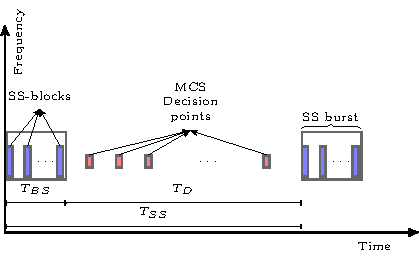
\includegraphics[width=0.7\columnwidth]{figures/chp_amc/amc_q_learning.pdf}}
\caption{Model of time scheduling of operations.}
\label{fig:amc-system-timing}
\end{figure}


During the data transmission window, the discret-time received signal for the $t$-th symbol period associated with the $k$-th fixed beam pair, is given by
\begin{equation}
\label{eq.:amc-rx-signal}
	\gls{not:Y}_{k,t} =
    \bar{\mathbf{w}}^H_k \,
  \channel _t\,
   \bar{\mathbf{f}}_k \,
   \gls{not:sscl}_t
   % _\userIdx
 +
  \bar{\mathbf{w}}^H_k \;
  \gls{not:Z}_t,
\end{equation}

\noindent where $\gls{not:sscl}$ is the symbol transmitted to the \ue, and $\gls{not:Z}_t$ is the additive white Gaussian noise with zero mean and variance \gls{not:var}.
%
%Note that the index $k$ and index $t$ refer to distinct points in time, i.e. the transmit and receive beams can have a mismatch with channel paths depending on \ue~mobility.
%
Defining
\begin{equation}
  \tilde{h}_{k,t} =     \bar{\mathbf{w}}^H_k \,
  \channel _t\,
   \bar{\mathbf{f}}_k \, ,
\end{equation}
as the effective channel at time $t$, associated with the chosen beam pair $\{ \bar{\mathbf{w}}_k, \bar{\mathbf{f}}_k \}$, the effective SNR at the \ue \, is given by
%
\begin{equation}
    \label{eq.:amc-snr}
    \textrm{SNR} = \frac{ \abs{
    % \hermitian{\gls{not:Wrx}\subArg{\userIdx}\argPair{:}{\idxI}}
     \tilde{h}_{k,t}
      % \subArg{\userIdx} \gls{not:Wtx}\subArg{\userIdx}\argPair{:}{\idxJ}
      }^2 }{\gls{not:var}} p_{\gls{not:sscl}},
\end{equation}
%https://www.overleaf.com/project/5d16668cdc29bf0ff4f11132
where $p_{\gls{not:sscl}}$ is the the power of transmitted symbol.
%
%
%\noindent with \gls{not:Wrx}\subArg{\userIdx}\argPair{:}{\idxI} and \gls{not:Wtx}\subArg{\userIdx}\argPair{:}{\idxJ} being the \idxI th and \idxJ th beams of the codebook  \gls{not:Wrx}\subArg{\userIdx} and \gls{not:Wtx}\subArg{\userIdx}, respectively.

% \subsection{Channel Description}
%The model in \eqref{eq.:rx_signal} assumes a narrowband block-fading channel, so the channel is almost constant within a time-frequency resource block \cite{alkhateeb2014}.

\subsection{Channel Model}

We assume a geometric channel model with limited number \gls{not:scatterers} of scatterers.
%
Each scatterer contributes with a single path between \gls{bs} and \gls{ue}. Therefore, the channel model can be expressed as
%
\begin{equation}\label{eq.:amc-channelModel}
\channel _t= \sqrt{\pathloss}\sum_{i=0}^{\gls{not:scatterers} - 1 } \gls{not:beta}_i \strRx \anglePair{i,t}{ue} \hermitian{\strTx  \anglePair{i,t}{bs}} e^{ \mathrm{j} 2 \pi f_i tT_s} ,
\end{equation}
\noindent where $T_s$ is the \gls{ofdm} symbol period, $\pathloss$ denotes the pathloss, \gls{not:beta} is the complex gain of the $k$th path and $f_i$ is the Doppler frequency for the $i$th path.
%
The parameters \azm~$\in$ \range{0}{2\pi} and \elev~$\in$ \range{0}{\pi} denote the azimuth and elevation angles at the \base \, (\gls{aod}) and the \ue \, (\gls{aoa}).
%
We assume a \gls{ura}, the response of which is written as:
%
\begin{equation*}
  \begin{split}
    \strTx \anglePair{i,t}{bs} = & \frac{1}{\sqrt{\gls{not:txAnt}}} \bigg[ 1, \expUraPhase{}{i,t}{bs}, \\ & \ldots ,\expUraPhase{(\gls{not:txAnt} -1 )}{i,t}{bs} \bigg],
  \end{split}
\end{equation*}
where \dist ~is the antenna element spacing, and \wave~is the signal wavelength. The array response at \gls{ue} can be written similarly.

The expression in \eqref{eq.:amc-channelModel} can be expressed compactly as
\begin{equation}
\label{eq.:amc-channelModelMtx}
\channel _t = \strRxMtx \diag{\gls{not:betaVec}_t} \hermitian{\strTxMtx},
\end{equation}
where $\gls{not:betaVec}_t = \left[ \gls{not:beta}_0 e^{ \mathrm{j} 2 \pi f_0 t T_s}, \ldots, \gls{not:beta}_{\gls{not:scatterers}-1} e^{ \mathrm{j} 2 \pi f_{S-1} t T_s} \right]$, and the matrices \strRxMtx~and \strTxMtx~are formed by the concatenation of array response vector at the \base~and \ue, respectively.

\subsection{Transmission Model}
\label{subsec:la-trans}
The transmission process takes into account the channel coding and modulation blocks.
%
In this work, we implement all the steps specified in the \gls{nr} channel coding block except the rate matching \cite{3gpp.38.212}.
%
The \gls{cb} segmentation divides the transport block of $n_{bits}$ bits to fit the input size accepted by the \gls{ldpc} encoder, padding whenever necessary.
%
At the \gls{mcs} decision points, shown in Figure \ref{fig:amc-system-timing}, the  \gls{ue} reports the measured \gls{cqi} to the \gls{bs}, which decides the \gls{mcs} accordingly.
%
The selected \gls{mcs} is informed to the \gls{ue} through the \gls{pdcch} as a part of the \gls{dci}. This process is shown in Figure \ref{fig:amc-system-model}.
%

We considered a subset of the \gls{mcs}s in Table 5.1.3.1-1 in \cite{3gpp.38.214}, from the \gls{mcs} indexes 3 to 27. For our \gls{rl} based solution, the \gls{cqi} is a quantized measure of the \gls{snr}, and the number of possible \gls{cqi}s is defined by $N_{\text{cqis}}$. The \gls{cqi} metric for the \gls{rl}-\gls{amc} is defined as:
\begin{equation}\label{eq:amc-cqi}
    \textrm{CQI} =
    \begin{cases}
    0, \text{if } \textrm{SNR} \leq \textrm{SNR}_{\text{min}}\\
    (N_{\text{cqi}}-1), \text{if } \textrm{SNR} \geq \textrm{SNR}_{\text{max}}\\
    \floor[\Big]{\frac{(\textrm{SNR} - \textrm{SNR}_{\text{min}})(N_{\text{cqi}}-1)}{\textrm{SNR}_{\text{max}}-\textrm{SNR}_{\text{min}}}}
    \end{cases}
\end{equation}
\noindent Note that each \gls{cqi}, except the minimum and the maximum ones, comprises \gls{snr} intervals having the same length.
% , since the \gls{snr} inside the range $[snr_{min},snr_{max}]$ is divided equally into \gls{cqi}s in this calculation.

At each \gls{tti} the \gls{bs} makes a transmission of a \gls{tb} of $n_{bits}$ at the chosen \gls{mcs}. The \gls{ue} receives a \gls{tb} from the \gls{bs} and, in possession of the chosen \gls{mcs}, decodes the \gls{tb} and calculates its \gls{ber}, \gls{bler} and spectral efficiency.
%
%The \gls{ber} is the Hamming distance between the decoded \gls{tb} and transmitted \gls{tb}.
%
% The \gls{bler} is a ratio of blocks with \gls{ber} above $0.1$. The spectral efficiency $\eta$, in $bit/s/Hz$, is calculated in terms of number of bits per modulation symbol \gls{not:mod} and the code rate \gls{not:rate} as:
The \gls{bler} is the ratio of incorrectly received blocks over the total number of received blocks. %where a block is the result of the code block segmentation.
%
The spectral efficiency $\eta$, in $bit/s/Hz$, is calculated as:
\begin{equation}
 \label{eq.:spec-eff}
 \eta = (1-\textrm{\gls{bler}})\gls{not:mod}\gls{not:rate} \, ,
\end{equation}
\noindent where \gls{not:mod} is the number of bits per modulation symbol and \gls{not:rate} is the code rate.

\begin{figure}[htb]
\centerline{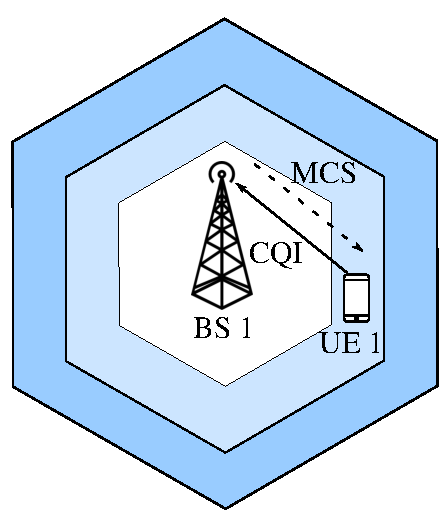
\includegraphics[width=0.4\columnwidth]{figures/chp_amc/system-model-mateus.pdf}}
\caption{Exchange of signals involved in the AMC procedure}
\label{fig:amc-system-model}
\end{figure}





%%%%%%%%%%%%%%%%%%%%%%%%%%%%%%%%%%--End Of Section--%%%%%%%%%%%%%%%%%%%%%%%%%%%%%%%%%%%%%

\section{Proposed Solution}

The proposed solution is a Q-learning based link adaptation scheme, herein referred to as \gls{ql-amc}.
%
In the proposed approach, the \gls{bs} selects the \gls{mcs} based on the state-action mapping obtained from the Q-learning algorithm.
%
More specifically, the \gls{bs} chooses the \gls{mcs} using the Q-table obtained from the \gls{rl} algorithm.
%
The \gls{rl} based solution enables the system to learn the particularities of the environment and adapt to it.

A diagram adapting the model from Figure \ref{fig:rlbasic} to the \gls{amc} problem is shown in Figure \ref{fig:amc-rl-frame}.
%
\begin{figure}[htb]
\centerline{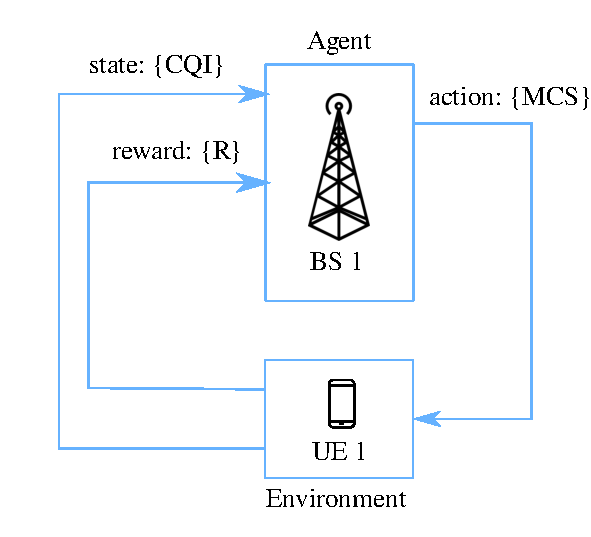
\includegraphics[width=0.5\columnwidth]{figures/chp_amc/rl-framework-mateus.pdf}}
\caption{Basic diagram of the proposed AMC scheme}
\label{fig:amc-rl-frame}
\end{figure}
%

In the proposed \gls{amc} problem, the state space is the set of all possible \gls{cqi}s, from $0$ to $(N_{\text{cqi}}-1)$; the action space is the set of all possible \gls{mcs}s. As for the reward, we consider two different metrics.
%
The first reward function is a non-linear one defined as:
\begin{equation}\label{eq.:rewardBler}
  R_1 = \begin{cases}
  \gls{not:mod} \gls{not:rate}, \text{ if } \textrm{BLER} \leq \textrm{BLER}_{\text{T}} \\
  -1, \text{ else.}
\end{cases}
\end{equation}
\noindent where \gls{not:mod} is the number of bits per modulation symbol, \gls{not:rate} is the code rate and $\textrm{BLER}_{\text{T}}$ is the target \gls{bler} of the system, $10\%$ in case of \gls{embb} \cite{3gpp.38.214}.
%
The goal of this reward function is to allow the agent to choose the best \gls{mcs} that satisfies the \gls{bler} target. The second reward is defined in terms of the spectral efficiency (in bits/second/hertz):
\begin{equation}\label{eq.:rewardSE}
    R_2 = (1-\textrm{BLER}) \gls{not:mod} \gls{not:rate} \text{.}
\end{equation}
\noindent With this function, the agent will try to maximize the spectral efficiency.
A summary of the proposed \gls{ql-amc} algorithm is shown in Algorithm \ref{amc-alg}.

\begin{algorithm}[htb]
  \caption{\strut QL-AMC}
    \label{amc-alg}
 \nonl Initialize $Q(s, a) = 0$, for all $s \in \mathcal{S}, a \in \mathcal{A}$\;
 \nonl \ForEach{MCS Decision Point (see Fig. \ref{fig:amc-system-timing})}{
  The UE \emph{observes the state} $s: $\gls{cqi} and feeds it back to the BS;\\
  The BS \emph{takes an action} $a: \textrm{MCS}$ using the policy driven by $Q$ (e.g., $\epsilon$-greedy);\\
  The BS \emph{perceives a reward} $r$ (c.f. Eqs. (\ref{eq.:rewardBler}) or (\ref{eq.:rewardSE})) and observes the next state $s^{\prime}$\;
  The BS update the Q-table: $Q(s, a) \leftarrow (1-\alpha) Q(s, a) + \alpha [r + \gamma \max_a Q(s',a)]$\;
  $s \leftarrow s^{\prime}$\;
\nonl }

\end{algorithm}


As will be shown in the next section, we will evaluate the impact and importance of on the system's \gls{bler} and spectral efficiency, and the difference between linear and non-linear rewards.

The Table \ref{tab:ql-amc-def} summarizes the definitions of state, action and reward.

\begin{table}[htb]
\centering
\caption{\gls{rl} elements}
\label{tab:ql-amc-def}
\begin{tabularx}{0.55\columnwidth}{X r}
\toprule
\textbf{Element} 	      & \textbf{Definition} \\
\midrule
State                   & \gls{cqi} \\
Action                  & \gls{mcs} \\
Reward                  & Eq: \eqref{eq.:rewardBler}, \eqref{eq.:rewardSE} \\
\bottomrule
\end{tabularx}
\end{table}
%

%%%%%%%%%%%%%%%%%%%%%%%%%%%%%%%%%%--End Of Section--%%%%%%%%%%%%%%%%%%%%%%%%%%%%%%%%%%%%%

\section{Simulations and Results}
\label{sec:amc-simulation}
\subsection{Simulation Parameters}
We assess the system performance with one \gls{bs} that serves one \gls{ue}.
%
The system has a bandwidth $B$ with a frequency carrier of $28$ GHz. Each resource block has a total of $12$ subcarriers and a subcarrier spacing $\gls{not:sub-spacing}= 120 \text{KHz}$.
%
%The frame is composed by 10 subframes, and each subframe is composed of multiple slots, where each slot has 14 symbols.
We consider the channel model defined in \eqref{eq.:amc-channelModel}.
%
The path loss follows a urban macro (UMa) model with non-line-of-sight (NLOS). Shadowing is modeled according to a log-normal distribution with standard deviation of $6$ dB \cite{AliZaidi632018}.
%
The noise power is fixed at $-123.185$ dBm.
%
A summary of the main simulation parameters is provided in Table~\ref{tab:amc-sim-params}, while the parameters of the proposed \gls{ql-amc} algortihm are listed in Table \ref{tab:amc-rl-params}.


\begin{table}[htb]
\centering
\caption{Simulation Parameters}
\label{tab:amc-sim-params}
\begin{tabularx}{0.8\columnwidth}{X r}
\toprule
\textbf{Parameter} 	& \textbf{Value} \\
\midrule
\gls{bs} height & 15 m\\
\gls{ue} height & 1.5 m\\
\gls{ue} track & rectilinear\\
\gls{bs}  antenna model & omnidirectional \\
\gls{bs}  antennas & 64 \\
\gls{ue} antenna model & omnidirectional \\
\gls{ue} antennas & 1 \\
Transmit power & 43 dBm\\
Frequency & 28 GHz\\
Bandwidth & 1440 MHz\\
Number of subcarriers  & 12\\
Subcarrier spacing & 120 kHz\\
Number of subframes & 10\\
Number of symbols & 14\\
Number of information bits per TTI & 1024\\
Azimuth angle spread & $[-60^{\circ}, 60^{\circ}]$\\
Azimuth angle mean & $0^{\circ}$\\
Elevation angle spread & $[60^{\circ}, 120^{\circ}]$\\
Elevation angle mean & $90^{\circ}$\\

Number of paths & 10\\
Path loss & UMa NLOS\\
Shadowing standard deviation & 6 dB\\
%Noise spectral density & -123 & dBm/Hz\\
\bottomrule
\end{tabularx}
\end{table}
%


\begin{table}[htb]
	\centering
	\caption{QL-AMC Parameters}
	\label{tab:amc-rl-params}
	\begin{tabularx}{0.8\columnwidth}{l r}
		\toprule
		\textbf{Parameter} 	   & \textbf{Value} \\
    \midrule
    $\textrm{SNR}_{\text{min}}$ for Eq. \eqref{eq:amc-cqi} & $-5$ \\
    $\textrm{SNR}_{\text{max}}$ for Eq. \eqref{eq:amc-cqi} & $40$ \\
		Discount factor ($\gamma$) & 0.10\\
		Learning rate ($\alpha$) & 0.90\\
		Maximum exploration rate ($\epsilon_{\max}$) & 0.50\\
    Minimum exploration rate ($\epsilon_{\min}$) & 0.05\\
    Cardinality of state space & $\{10,15,30,60 \}$\\
		\bottomrule
	\end{tabularx}
\end{table}

\subsection{Baseline Solutions}

% We compare the \gls{ql-amc} against the \gls{amc} based on the channel state \cite{fantacci2009adaptive} and target \gls{bler}, which produces a look-up table and also against the \gls{olla} technique \cite{Sarret2015}.
%
We compare the \gls{ql-amc} against the \gls{amc} based on a fixed look-up table \cite{fantacci2009adaptive} and also against the \gls{olla} technique from \cite{Pedersen2007}.
% We consider two fixed \gls{mcs}, the first is the QPSK with code rate of $1/3$ and the second is 16\gls{qam} with rate of $2/3$. In the results they are referred as "fixed 1" and "fixed 2".
%
In the fixed look-up table approach, a static mapping of \gls{snr} to \gls{cqi} is obtained by analyzing the \gls{bler} curves and selecting the best \gls{mcs}, in terms of throughput, that satisfies the target \gls{bler} \cite{bruno2014robust}.
%
The process of analyzing the \gls{bler} curves gives the \gls{snr} thresholds that separate each \gls{cqi}, as such the \gls{snr} to \gls{cqi} mapping for the look-up table and the \gls{olla} algorithm is different from the \gls{ql-amc} defined in Eq. \eqref{eq:amc-cqi}.
%
We assumed a direct mapping of \gls{cqi} to \gls{mcs}, i.e., each \gls{cqi} is mapped to one \gls{mcs} only .
% \begin{table}[tb]
% \centering
% \caption{Look-up Table}
% \label{tab:look-up}
% \begin{tabularx}{0.5\columnwidth}{l X r}
% \toprule
%  CQI   & Modulation   & Rate \\
% \midrule
%  0     & QPSK         & 1/3   \\
%  1     & QPSK         & 1/2   \\
%  2     & QPSK         & 2/3   \\
%  3     & 16QAM        & 1/2   \\
%  4     & 16QAM        & 2/3   \\
%  5     & 16QAM        & 3/4   \\
%  6     & 64QAM        & 2/3   \\
%  7     & 64QAM        & 3/4   \\
%  8     & 64QAM        & 5/6   \\
% \bottomrule
% \end{tabularx}
% \end{table}
The \gls{olla} technique consists of improving the conventional MCS look-up table by adjusting the \gls{snr} thresholds according to the \gls{acknack} from previous transmissions.
%
This adjustment is made by adding an offset to the estimated \gls{snr} to correct the \gls{mcs}s.
%
The \gls{snr} that is transformed to \gls{cqi} is:
\begin{equation}
\textrm{SNR}_{\text{olla}} = \textrm{SNR} + \Delta_{\text{olla}}
\end{equation}
\noindent where the $\Delta_{olla}$ is updated at each time step according to the Eq. \eqref{eq.:olla} \cite{Blanquez-Casado2016}:
\begin{equation}\label{eq.:olla}
  \Delta_{\text{olla}} \leftarrow \Delta_{\text{olla}} + \Delta_{\text{up}} \cdot e_{\text{blk}} - \Delta_{\text{down}} \cdot (1 - e_{\text{blk}}),
\end{equation}
\noindent where $e_{\text{blk}} = 1$ in case of NACK, or $e_{\text{blk}} = 0$ if the transmission is successful.
%
The parameters $\Delta_{\text{up}}$, $\Delta_{\text{down}}$ and the target \gls{bler}, $\textrm{BLER}_{\text{T}}$, are inter-related. In fact, by fixing the $\Delta_{\text{up}}$ and the $\textrm{BLER}_{\text{T}}$, the $\Delta_{\text{down}}$ can be calculated as \cite{Pedersen2007}:
$$
\Delta_{\text{down}} = \frac{\Delta_{\text{up}}}{\frac{1}{\textrm{BLER}_{\text{T}}} -1}.
$$
The target \gls{bler} for the \gls{olla} algorithm is fixed at $0.1$, while we assume three values for $\Delta_{\text{up}}$: 0.01dB, 0.1dB and  1dB.

\subsection{Experiment Description and Results}

The experiment devised to assess the performance of the \gls{ql-amc} in comparison to the baseline solutions (look-up table and OLLA) is composed of two phases, namely the learning phase and the deployment phase.
%
We also evaluate the effect of the type of reward function considered (i.e., Eqs. \eqref{eq.:rewardBler} or \eqref{eq.:rewardSE}), and the different number of \gls{cqi}s. As such, each \gls{ql-amc} configuration is defined in terms of the cardinality of the state space and the reward function.
%
The action space is the set of all possible modulations orders and code rates, being the same for all configurations.


\subsubsection{Learning Phase}
In the first phase, the \gls{rl} agent populates the Q-table to learn the environment.
%
Each configuration of the \gls{ql-amc} passes through this phase only one time. Our simulation time starts with the \gls{ue} positioned at a radial distance of $20m$ from the \gls{bs}. The UE moves away from the \gls{bs} up to a distance of 100m. Then, the \gls{ue} comes back to its original position following the same path in the reverse direction.
%
The \gls{ue} has a speed of $5km/h$ and the simulation runs for a time equivalent to $160s$ of the network time, which corresponds to the transmission of 32.000 frames.
%


%
The Table \ref{tab:amc-train-results} summarizes the results, providing average values, of the metrics for each configuration of the \gls{ql-amc}.
%
SE is the spectral efficiency given by Equation \eqref{eq.:spec-eff}.
%
\begin{table}[htb]
\centering
\caption{Training Phase Results}
\label{tab:amc-train-results}
\begin{tabularx}{0.75\columnwidth}{l X X X r}
\toprule
Length & Reward &  BLER &  SE &   BER \\
\midrule
10 &           2 & 0.0270 &  5.0850 & 0.0065 \\
10 &           3 & 0.0288 &  5.1696 & 0.0070 \\
15 &           2 & 0.0263 &  5.0827 & 0.0065 \\
15 &           3 & 0.0289 &  5.1054 & 0.0071 \\
30 &           2 & 0.0264 &  5.1463 & 0.0065 \\
30 &           3 & 0.0286 &  5.1227 & 0.0070 \\
60 &           2 & 0.0283 &  5.0852 & 0.0068 \\
60 &           3 & 0.0279 &  5.1701 & 0.0068 \\
\bottomrule
\end{tabularx}
\end{table}

Table \ref{tab:amc-train-results} reveals that configurations adopting the spectral efficiency (reward 2) as the reward function, with state space of lengths 10 or 60, achieve the best results in terms of spectral efficiency.
%
This is coherent since reward 2 is the own spectral efficiency.
%
When the performance metric is the \gls{bler}, the non-linear reward function (reward 1, Eq. \eqref{eq.:rewardBler}) provides the best results with lengths of 15 and 30.
%
Figures \ref{fig:amc-train-spceff} and \ref{fig:amc-train-bler} shows respectively the average spectral efficiency and the average \gls{bler} of these four possible configurations.
%
Figure \ref{fig:amc-train-spceff} shows that the length of the state space indeed has an important influence on the learning speed.
%
The smaller the length is, the faster is the learning speed, as expected.
%
The \gls{ql-amc} with length 60 has the worst performance before $10s$, but after $20s$ the performance of all configurations is approximately the same.
%

\begin{figure}[!htbp]
\centerline{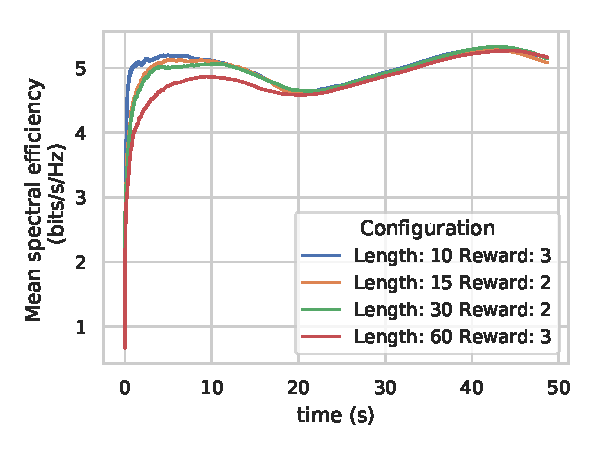
\includegraphics[width=0.7\columnwidth]{figures/chp_amc/Spec-Eff-Train.pdf}}
\caption{Mean spectral efficiency on training phase}
\label{fig:amc-train-spceff}
\end{figure}

\begin{figure}[!htbp]
\centerline{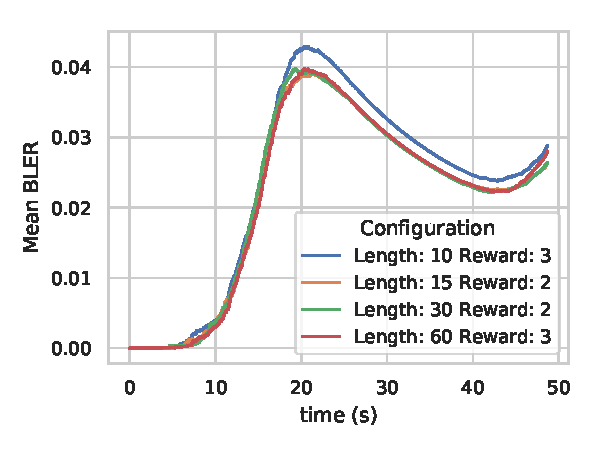
\includegraphics[width=0.7\columnwidth]{figures/chp_amc/BLER-Train.pdf}}
\caption{Mean \gls{bler} on training phase}
\label{fig:amc-train-bler}
\end{figure}

The performances of the \gls{ql-amc}s in terms of \gls{bler} are similar for all configurations in Figure \ref{fig:amc-train-bler}.
%
Before the $20s$ mark the curves are close, whereas the configuration with length 10 degrades slightly compared to other configurations after this time mark.


\subsubsection{Deployment phase}
The second phase uses the knowledge from the first phase, but with an $\epsilon$-greedy policy with a fixed value of $\epsilon = 0.05$, accordingly to the minimum value of the $\epsilon$-decreasing in the training phase.
%
The goal is to have an assessment of how the \gls{rl} agent performs in the long run.
%

In the deployment phase, we compare the proposed \gls{ql-amc} solution with the baseline solutions (look-up table and OLLA).
%
We perform $200$ Monte Carlo runs. At each run, the \gls{ue} starts at a random position between $25m$ and $90m$ of the \gls{bs}.
%
The \gls{ue} moves in a random rectilinear direction with a random speed between $10km/h$ and $20km/h$. This corresponds to a total of $K=125$ frames. Recall that each frame comprises a beam sweeping procedure, followed by data transmission jointly with a MCS selection procedure, as shown in Figure \ref{fig:amc-system-timing}.
%


Table \ref{tab:amc-deploy-results} summarizes the results in the deployment phase in terms of average values for each configuration of the \gls{ql-amc} and baseline solution.
%
The first column represents the type of solution adopted.
%
% The two fixed \gls{mcs} schemes (denoted as "Fixed 1" and "Fixed 2") consider QPSK with code rate of 1/3 and 16QAM with code rate of 2/3, respectively.
%
We consider three \gls{olla} schemes, denoted as \gls{olla} 1, 2 and 3, which consider $\Delta_{\text{up}}$ 0.01dB, 0.1dB and 1dB, respectively.
%
The conventional \gls{amc} with a fixed look-up table is denoted as "Table".
%
The second column represents the number of \gls{cqi}s and the type column represents the reward function used, defined by Eqs. \eqref{eq.:rewardBler}, \eqref{eq.:rewardSE}, and denoted as \gls{bler} and SE.
%

\begin{table}[tb]
\centering
\caption{Deployment Phase Results (Average over 200 runs)}
\label{tab:amc-deploy-results}
\begin{tabularx}{\columnwidth}{l X X X X r}
  \toprule
  Type    & Cardinality &      Reward  &  BLER &     SE  &    BER \\
  \midrule
   QL-AMC &     10 &           BLER   & 0.0320 &  3.6700 & 0.0088 \\
   QL-AMC &     15 &           BLER   & 0.0306 &  3.3238 & 0.0087 \\
   QL-AMC &     30 &           BLER   & 0.0302 &  3.5594 & 0.0087 \\
   QL-AMC &     60 &           BLER   & 0.0306 &  3.8783 & 0.0087 \\
   QL-AMC &     10 &           SE     & 0.0306 &  3.9187 & 0.0086 \\
   QL-AMC &     15 &           SE     & 0.0301 &  3.8207 & 0.0085 \\
   QL-AMC &     30 &           SE     & 0.0310 &  3.9922 & 0.0086 \\
   QL-AMC &     60 &           SE     & 0.0311 &  4.1553 & 0.0086 \\
    Table &      - &           -      & 0.0311 &  3.8704 & 0.0088 \\
   OLLA 1 &      - &           -      & 0.0309 &  3.6700 & 0.0088 \\
   OLLA 2 &      - &           -      & 0.0330 &  1.8511 & 0.0090 \\
   OLLA 3 &      - &           -      & 0.0343 &  0.9999 & 0.0092 \\
  \bottomrule
\end{tabularx}
\end{table}

Analyzing Table \ref{tab:amc-deploy-results}, we see that the two \gls{ql-amc} configurations presenting the best results in terms of spectral efficiency are those with cardinality 30 and 60, adopting the reward function $R_1$ of Eq. \eqref{eq.:rewardSE}.
% %
% The knowledge learned in the training phase is passed through to the deployment phase, as these two configurations already demonstrated the best performance in the training phase.
%

\begin{figure}[tb]
\centerline{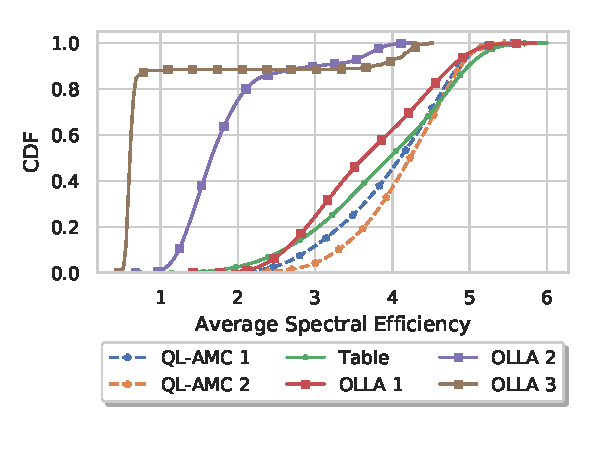
\includegraphics[width=0.7\columnwidth]{figures/chp_amc/SpecEff-Deploy.pdf}}
\vspace{-2ex}
\caption{CDF of average spectral efficiency (bps/Hertz)}
\label{fig:amc-dep-spceff}
\end{figure}

Figure \ref{fig:amc-dep-spceff} shows the cumulative distribution of the average spectral efficiency, in each Monte Carlo run, for the different \gls{ql-amc} configurations, with cardinality 30 and 60, which are labeled \gls{ql-amc} 1 and 2, respectively. We consider the reward function $R_2$ defined in Eq. \eqref{eq.:rewardSE}.
It can be seen that the proposed \gls{ql-amc} algorithm outperforms the baseline solutions in terms of spectral efficiency.
%comparison against to the baseline solutions.



%%%%%%%%%%%%%%%%%%%%%%%%%%%%%%%%%%--End Of Section--%%%%%%%%%%%%%%%%%%%%%%%%%%%%%%%%%%%%%


\section{Conclusions and Perspectives}
\label{sec:amc-conclusion}
We demonstrate through simulations that the \gls{rl} provides a self-exploratory framework that enables the \base~ to choose a suitable \gls{mcs} that maximizes the spectral efficiency.
%
Basically, the \gls{bs} decides a specific \gls{mcs} at a certain time instant. The \ue~ measures the reward of that action and report it to the \base.
%
Comparing with the fixed look-up table and \gls{olla} solutions, the proposed QL-AMC solution has achieved higher spectral efficiencies and lower BLERs.
%
Between the two rewards considered, the second one that is in function of the spectral efficiency has achieved the best performance.
%
As a perspective, we highlight extensions to multi-layer MIMO transmission. Moreover, a comparison with other RL-based algorithms such as multi-armed bandits (MABs) \cite{zhou2015survey} or deep RL solutions \cite{DeepRLSurvey} is envisioned.
%
% When considering multi-layer transmission, our \gls{rl}-based solution should be adapted to select both the \gls{amc} scheme and the number of spatial layers.
% %
% It is also worth mentioning that different spatial layers are associated with different \gls{cqi}s, which increases the number of possible actions and states of the proposed \gls{rl}-based \gls{amc} solution.
% %
% Hence, deep reinforcement learning should be investigated to deal with this increase in complexity.
%
% In addition, since \gls{nr} is a beam-based system, including the beam domain is another perspective.
% %
% In other words, our \gls{rl}-based solutions can also incorporate the selection of the best beam to transmit/receive data, among a set of choices (codebook).
% %
% These perspectives will be addressed in a follow-up work.

%%%%%%%%%%%%%%%%%%%%%%%%%%%%%%%%%%%%%%%%%%%%%%%%%%%%%%%%%%%%%%%%%%%%%%%%%%%%%%%%
